\newpage
% ============================================================
\subsection*{Actividad 6: Dependencia de rango largo en tráfico transaccional Cloud}
% ============================================================

Para la sexta actividad, nos sumergimos en el análisis de tráfico transaccional de la NASA, un dataset clásico que ha sido estudiado durante décadas por su riqueza y complejidad. Este tráfico no es solo un flujo de datos: es un reflejo de cómo los usuarios interactúan con la web, cómo las páginas se cargan, y cómo los servidores responden a esas demandas.

\subsubsection*{El problema: ¿Por qué el tráfico web NO se comporta como una fila de supermercado?}

Supongamos una autopista. Si el tráfico fuera Poisson, sería como si cada auto decidiera entrar a la ruta completamente al azar, sin importar lo que pase adelante. No habría tacos, no habría ráfagas: solo autos espaciados como gotas de lluvia en un día de llovizna suave.

Pero en la realidad, ¿qué pasa? Hay horas pico, hay accidentes que generan tacos de 5 km, hay ráfagas de autos que vienen todos juntos después de que se abre una barrera. El tráfico web es EXACTAMENTE igual.

Cuando un usuario pide una página de la NASA, no viene solo. Viene con imágenes, con scripts, con requests en cascada. Y si hay mucha gente conectada, se generan ráfagas (bursts) que el modelo Poisson no puede explicar. Poisson asume que cada evento es independiente, sin memoria del pasado. Pero la web tiene memoria: si hubo mucho tráfico hace un ratito, probablemente siga habiendo mucho tráfico ahora. Esa ``memoria'' es lo que llamamos dependencia de rango largo (LRD).

\begin{figure}[H]
    \centering
    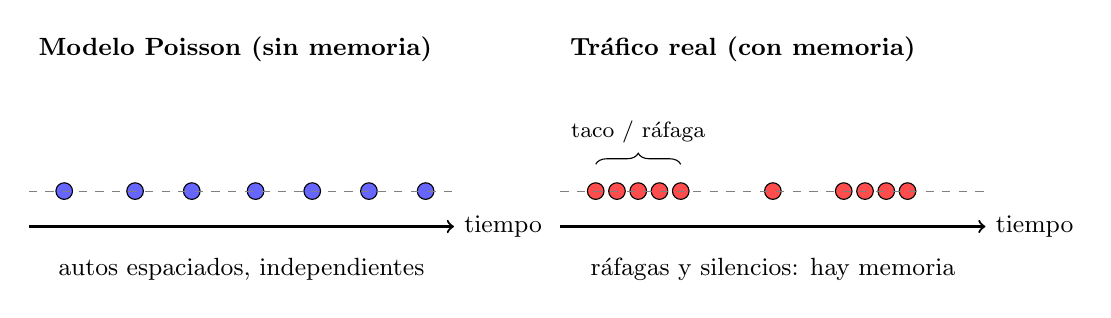
\begin{tikzpicture}[scale=0.9, every node/.style={font=\small}]
        % Panel izquierdo: Poisson (uniforme)
        \node[anchor=west] at (0,2.5) {\textbf{Modelo Poisson (sin memoria)}};
        \draw[thick,->] (0,0) -- (6,0) node[right] {tiempo};
        \foreach \x in {0.5,1.5,2.3,3.2,4.0,4.8,5.6} {
            \node[draw,circle,fill=blue!60,minimum size=6pt,inner sep=0] at (\x,0.5) {};
        }
        \draw[dashed,gray] (0,0.5) -- (6,0.5);
        \node at (3,-0.6) {autos espaciados, independientes};

        % Panel derecho: Real (bursty)
        \node[anchor=west] at (7.5,2.5) {\textbf{Tráfico real (con memoria)}};
        \draw[thick,->] (7.5,0) -- (13.5,0) node[right] {tiempo};
        % Ráfaga
        \foreach \x in {8.0,8.3,8.6,8.9,9.2} {
            \node[draw,circle,fill=red!70,minimum size=6pt,inner sep=0] at (\x,0.5) {};
        }
        % Espacio
        \node[draw,circle,fill=red!70,minimum size=6pt,inner sep=0] at (10.5,0.5) {};
        % Otra ráfaga
        \foreach \x in {11.5,11.8,12.1,12.4} {
            \node[draw,circle,fill=red!70,minimum size=6pt,inner sep=0] at (\x,0.5) {};
        }
        \draw[dashed,gray] (7.5,0.5) -- (13.5,0.5);
        % taco label
        \draw[decorate,decoration={brace,amplitude=4pt,raise=2pt}] (8.0,0.8) -- (9.2,0.8)
            node[midway,above=6pt,font=\footnotesize] {taco / ráfaga};
        \node at (10.5,-0.6) {ráfagas y silencios: hay memoria};
    \end{tikzpicture}
    \caption{Poisson asume independencia total (izquierda). El tráfico real exhibe ráfagas porque ``si hay taco, sigue habiendo taco'' (derecha).}
    \label{fig:a6-concepto-poisson}
\end{figure}

La Figura~\ref{fig:a6-serie} presenta la serie de tiempo real extraída del log NASA: $975\,721$ observaciones con media $\mu = 2{,}7450$~s, mediana $1{,}0000$~s y desviación estándar $137{,}6685$~s. Las ráfagas saltan a la vista.

\begin{figure}[H]
    \centering
    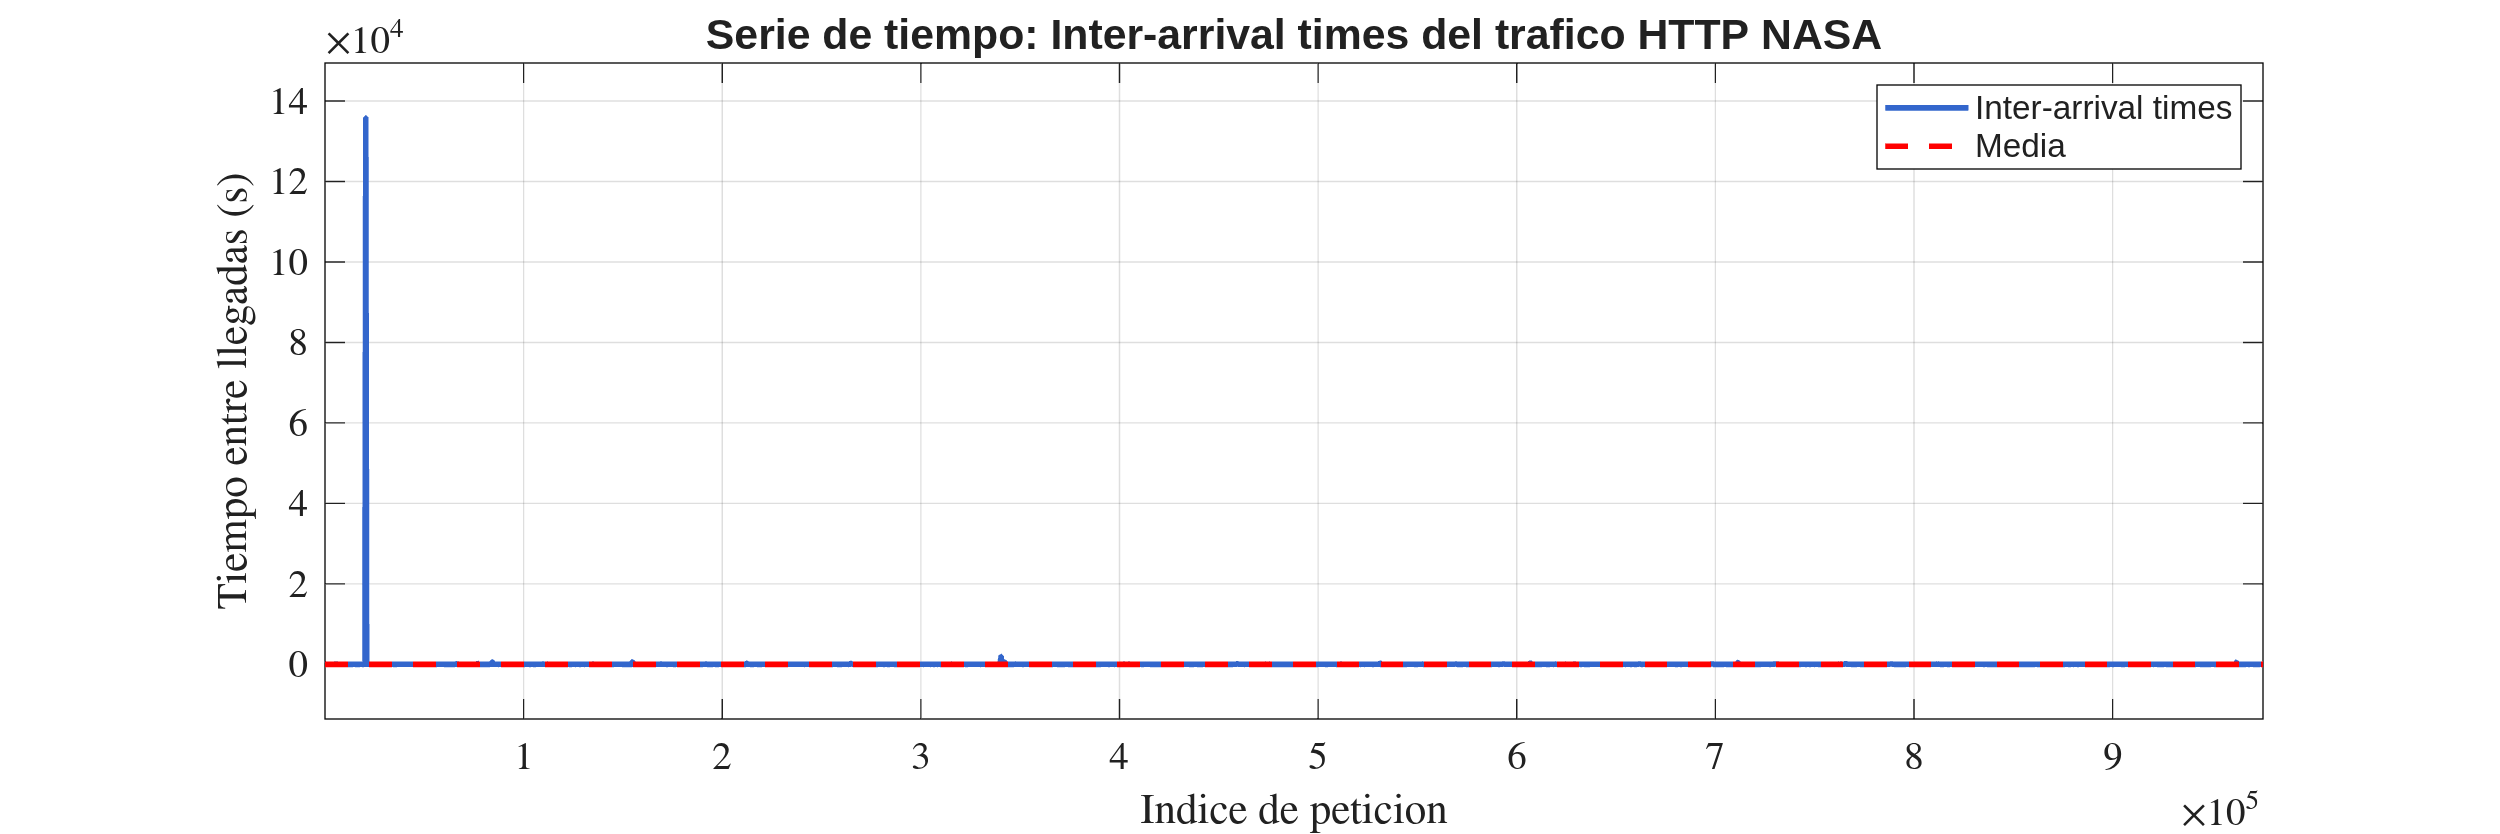
\includegraphics[width=\textwidth]{actividades/actividad6/imgs/serie_tiempo.png}
    \caption{Serie de tiempo de los inter-arrival times del tráfico HTTP NASA. La línea roja discontinua marca la media ($\mu = 2{,}7450$~s).}
    \label{fig:a6-serie}
\end{figure}

La Figura~\ref{fig:a6-histograma} compara la distribución empírica con la exponencial teórica de Poisson. La cola pesada y la concentración en valores bajos demuestran que Poisson no alcanza.

\begin{figure}[H]
    \centering
    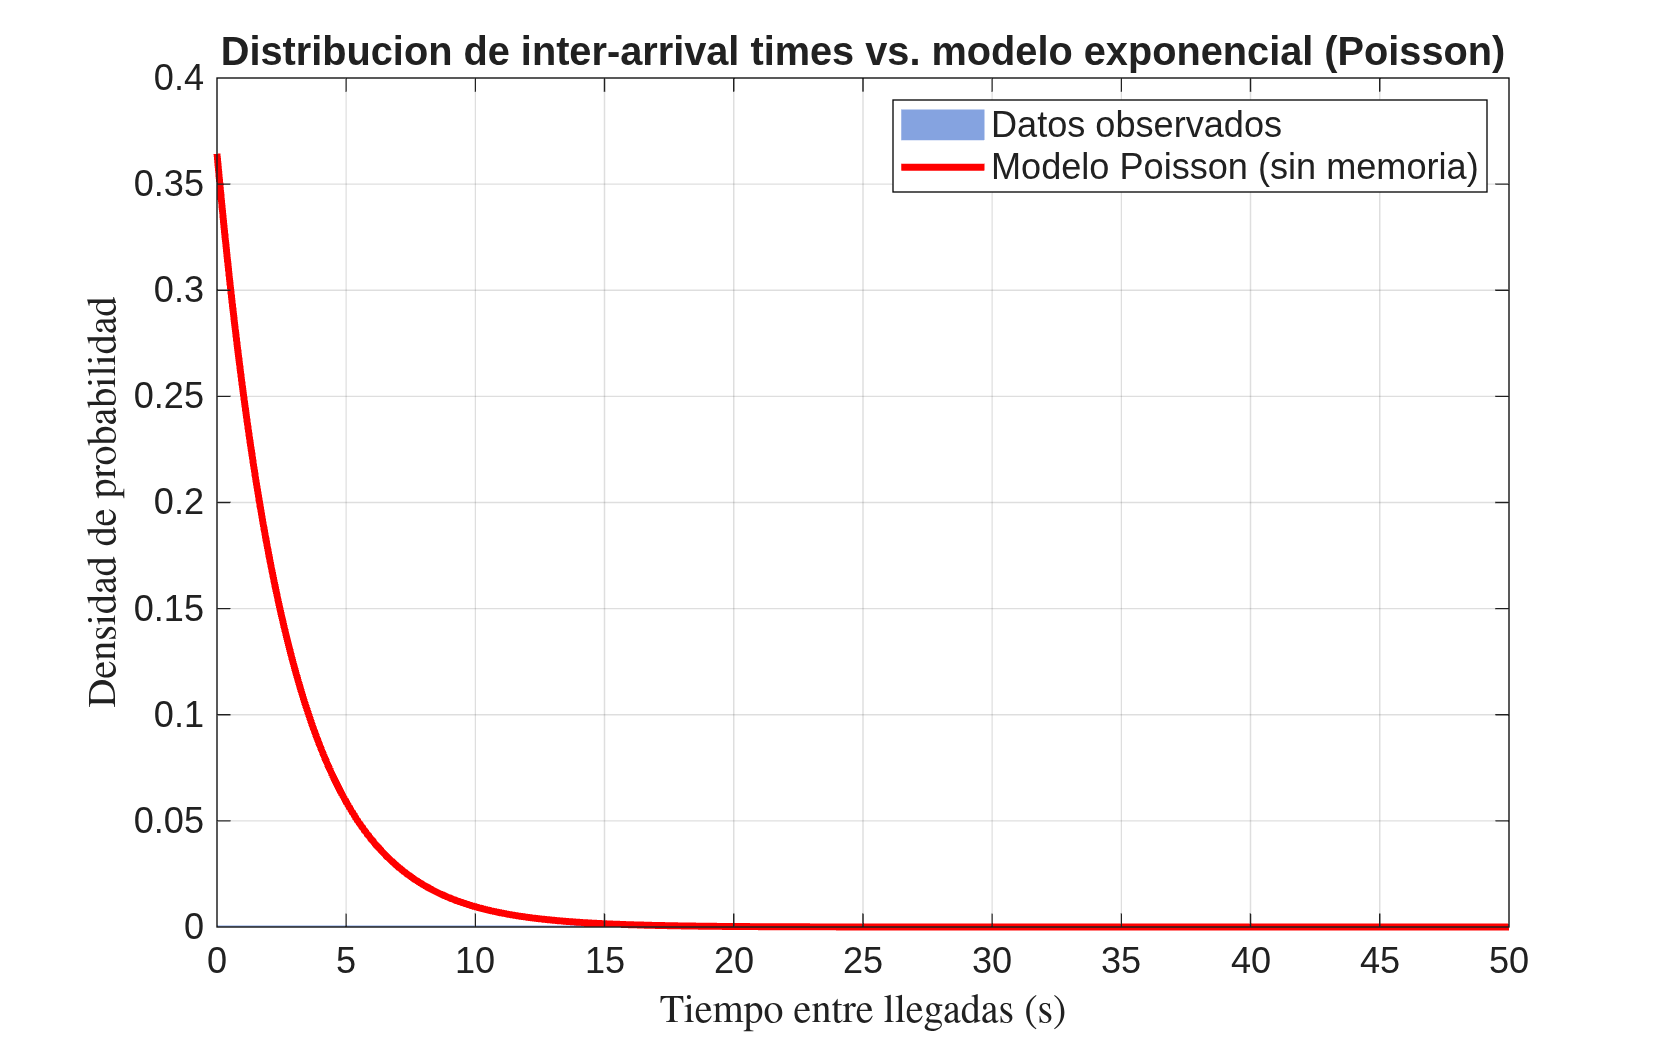
\includegraphics[width=0.85\textwidth]{actividades/actividad6/imgs/histograma.png}
    \caption{Histograma de inter-arrival times vs.~distribución exponencial teórica (Poisson). Las colas pesadas invalidan el modelo sin memoria.}
    \label{fig:a6-histograma}
\end{figure}

\subsubsection*{La solución: El parámetro de Hurst y la ``memoria'' del tráfico}

¿Cómo medimos esa ``memoria''? Acá entra el parámetro de Hurst ($H$), que el hidrólogo Harold Edwin Hurst usó en los años 50 para estudiar las crecidas del Nilo.

$H$ es un número entre 0 y 1 que indica qué tan persistente es una serie temporal:

\begin{itemize}[leftmargin=2em]
    \item $H = 0{,}5$: proceso Browniano, sin memoria. Cada paso es independiente. Es el mundo Poisson.
    \item $0{,}5 < H < 1$: dependencia de rango largo. Si el tráfico estuvo alto, tiende a seguir alto. Efecto ``si hay taco, sigue habiendo taco''.
    \item $0 < H < 0{,}5$: anti-persistencia. Si estuvo alto, tiende a bajar (muy raro en tráfico web).
\end{itemize}

\begin{figure}[H]
    \centering
    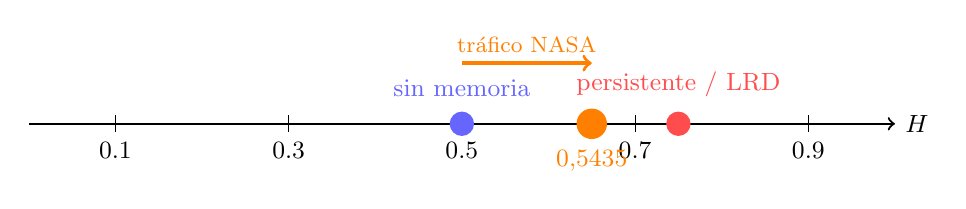
\begin{tikzpicture}[scale=1.1, every node/.style={font=\small}]
        % Escala
        \draw[thick,->] (0,0) -- (10,0) node[right] {$H$};
        \foreach \x/\label in {1/0.1, 3/0.3, 5/0.5, 7/0.7, 9/0.9} {
            \draw (\x,0.1) -- (\x,-0.1) node[below] {\label};
        }
        % Marcas de referencia
        \fill[blue!60] (5,0) circle (4pt);
        \node[above,blue!60] at (5,0.2) {sin memoria};

        \fill[red!70] (7.5,0) circle (4pt);
        \node[above,red!70] at (7.5,0.2) {persistente / LRD};

        % Flecha del tráfico NASA
        \draw[->,very thick,orange] (5,0.7) -- (6.5,0.7) node[midway,above,font=\footnotesize] {tráfico NASA};
        \fill[orange] (6.5,0) circle (5pt);
        \node[below,orange] at (6.5,-0.2) {$0{,}5435$};
    \end{tikzpicture}
    \caption{Escala del parámetro de Hurst. El tráfico NASA cae en la zona de memoria persistente ($H > 0{,}5$).}
    \label{fig:a6-escala-hurst}
\end{figure}

En nuestro análisis encontramos $H = 0{,}5435$, con un ajuste impecable ($R^2 = 0{,}9911$) e intervalo de confianza del 95\,\% $[0{,}5408;\,0{,}5462]$. Conclusión: el tráfico NASA tiene memoria, tiene ráfagas estructuradas y NO se puede modelar con Poisson.

\subsubsection*{Método 1: Varianza--Tiempo --- ``¿Qué tan predecible es el caos?''}

La idea del método VT es simple: agrupamos los datos en bloques cada vez más grandes y miramos cómo decae la varianza.

Imaginate la serie minuto a minuto (muchos bloques chicos), después de a 10 minutos (bloques medianos) y de a 100 minutos (bloques grandes). En un proceso Poisson, la varianza baja de forma predecible: se divide por el tamaño del bloque. Es como promediar números al azar: cuantos más promediés, más estable se vuelve el resultado.

Pero en un proceso con LRD, la varianza baja más lento. ¿Por qué? Porque los bloques grandes todavía tienen ``memoria'' entre sí. La ráfaga que empezó en el primer minuto sigue influyendo en el minuto 50. Entonces, agrupar no ``apaga'' la variabilidad tan rápido.

\begin{figure}[H]
    \centering
    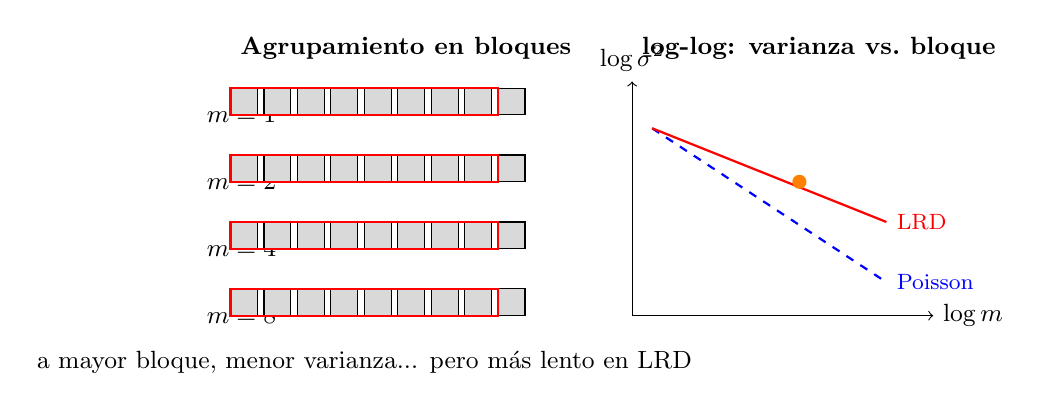
\begin{tikzpicture}[scale=0.85, every node/.style={font=\small}]
        % Panel izquierdo: agrupamiento
        \node[anchor=west] at (0,4.5) {\textbf{Agrupamiento en bloques}};
        \foreach \y/\label in {3.5/1,2.5/2,1.5/4,0.5/8} {
            \node[right] at (-0.5,\y) {$m=\label$};
            \foreach \x in {0,0.5,...,4} {
                \draw[fill=gray!30] (\x,\y) rectangle (\x+0.4,\y+0.4);
            }
            \draw[thick,red] (0,\y) rectangle (4,\y+0.4);
        }
        \node at (2,-0.2) {a mayor bloque, menor varianza... pero más lento en LRD};

        % Panel derecho: mini gráfico log-log
        \begin{scope}[shift={(6,0.5)}]
            \node[anchor=west] at (0,4) {\textbf{log-log: varianza vs.~bloque}};
            \draw[->] (0,0) -- (4.5,0) node[right] {\small $\log m$};
            \draw[->] (0,0) -- (0,3.5) node[above] {\small $\log \sigma^2$};
            % Recta Poisson (más empinada)
            \draw[thick,blue,dashed] (0.3,2.8) -- (3.8,0.5) node[right,font=\footnotesize] {Poisson};
            % Recta LRD (menos empinada)
            \draw[thick,red] (0.3,2.8) -- (3.8,1.4) node[right,font=\footnotesize] {LRD};
            % Punto NASA
            \fill[orange] (2.5,2.0) circle (3pt);
        \end{scope}
    \end{tikzpicture}
    \caption{VT agrupa en bloques crecientes (izquierda). En log-log, la pendiente de LRD es menos empinada porque la varianza decae más lento (derecha).}
    \label{fig:a6-concepto-vt}
\end{figure}

El script \texttt{vt.m} hace exactamente eso: agrupa en $m = 1, 2, 4, 8, \dots$, calcula la varianza de cada agregación y grafica $\log(\text{varianza})$ vs.~$\log(m)$. La pendiente de esa recta nos da $H$.

Resultado: $\hat{H} = 0{,}5435$ con $R^2_{\text{VT}} = 0{,}9911$. LRD confirmada.

\begin{figure}[H]
    \centering
    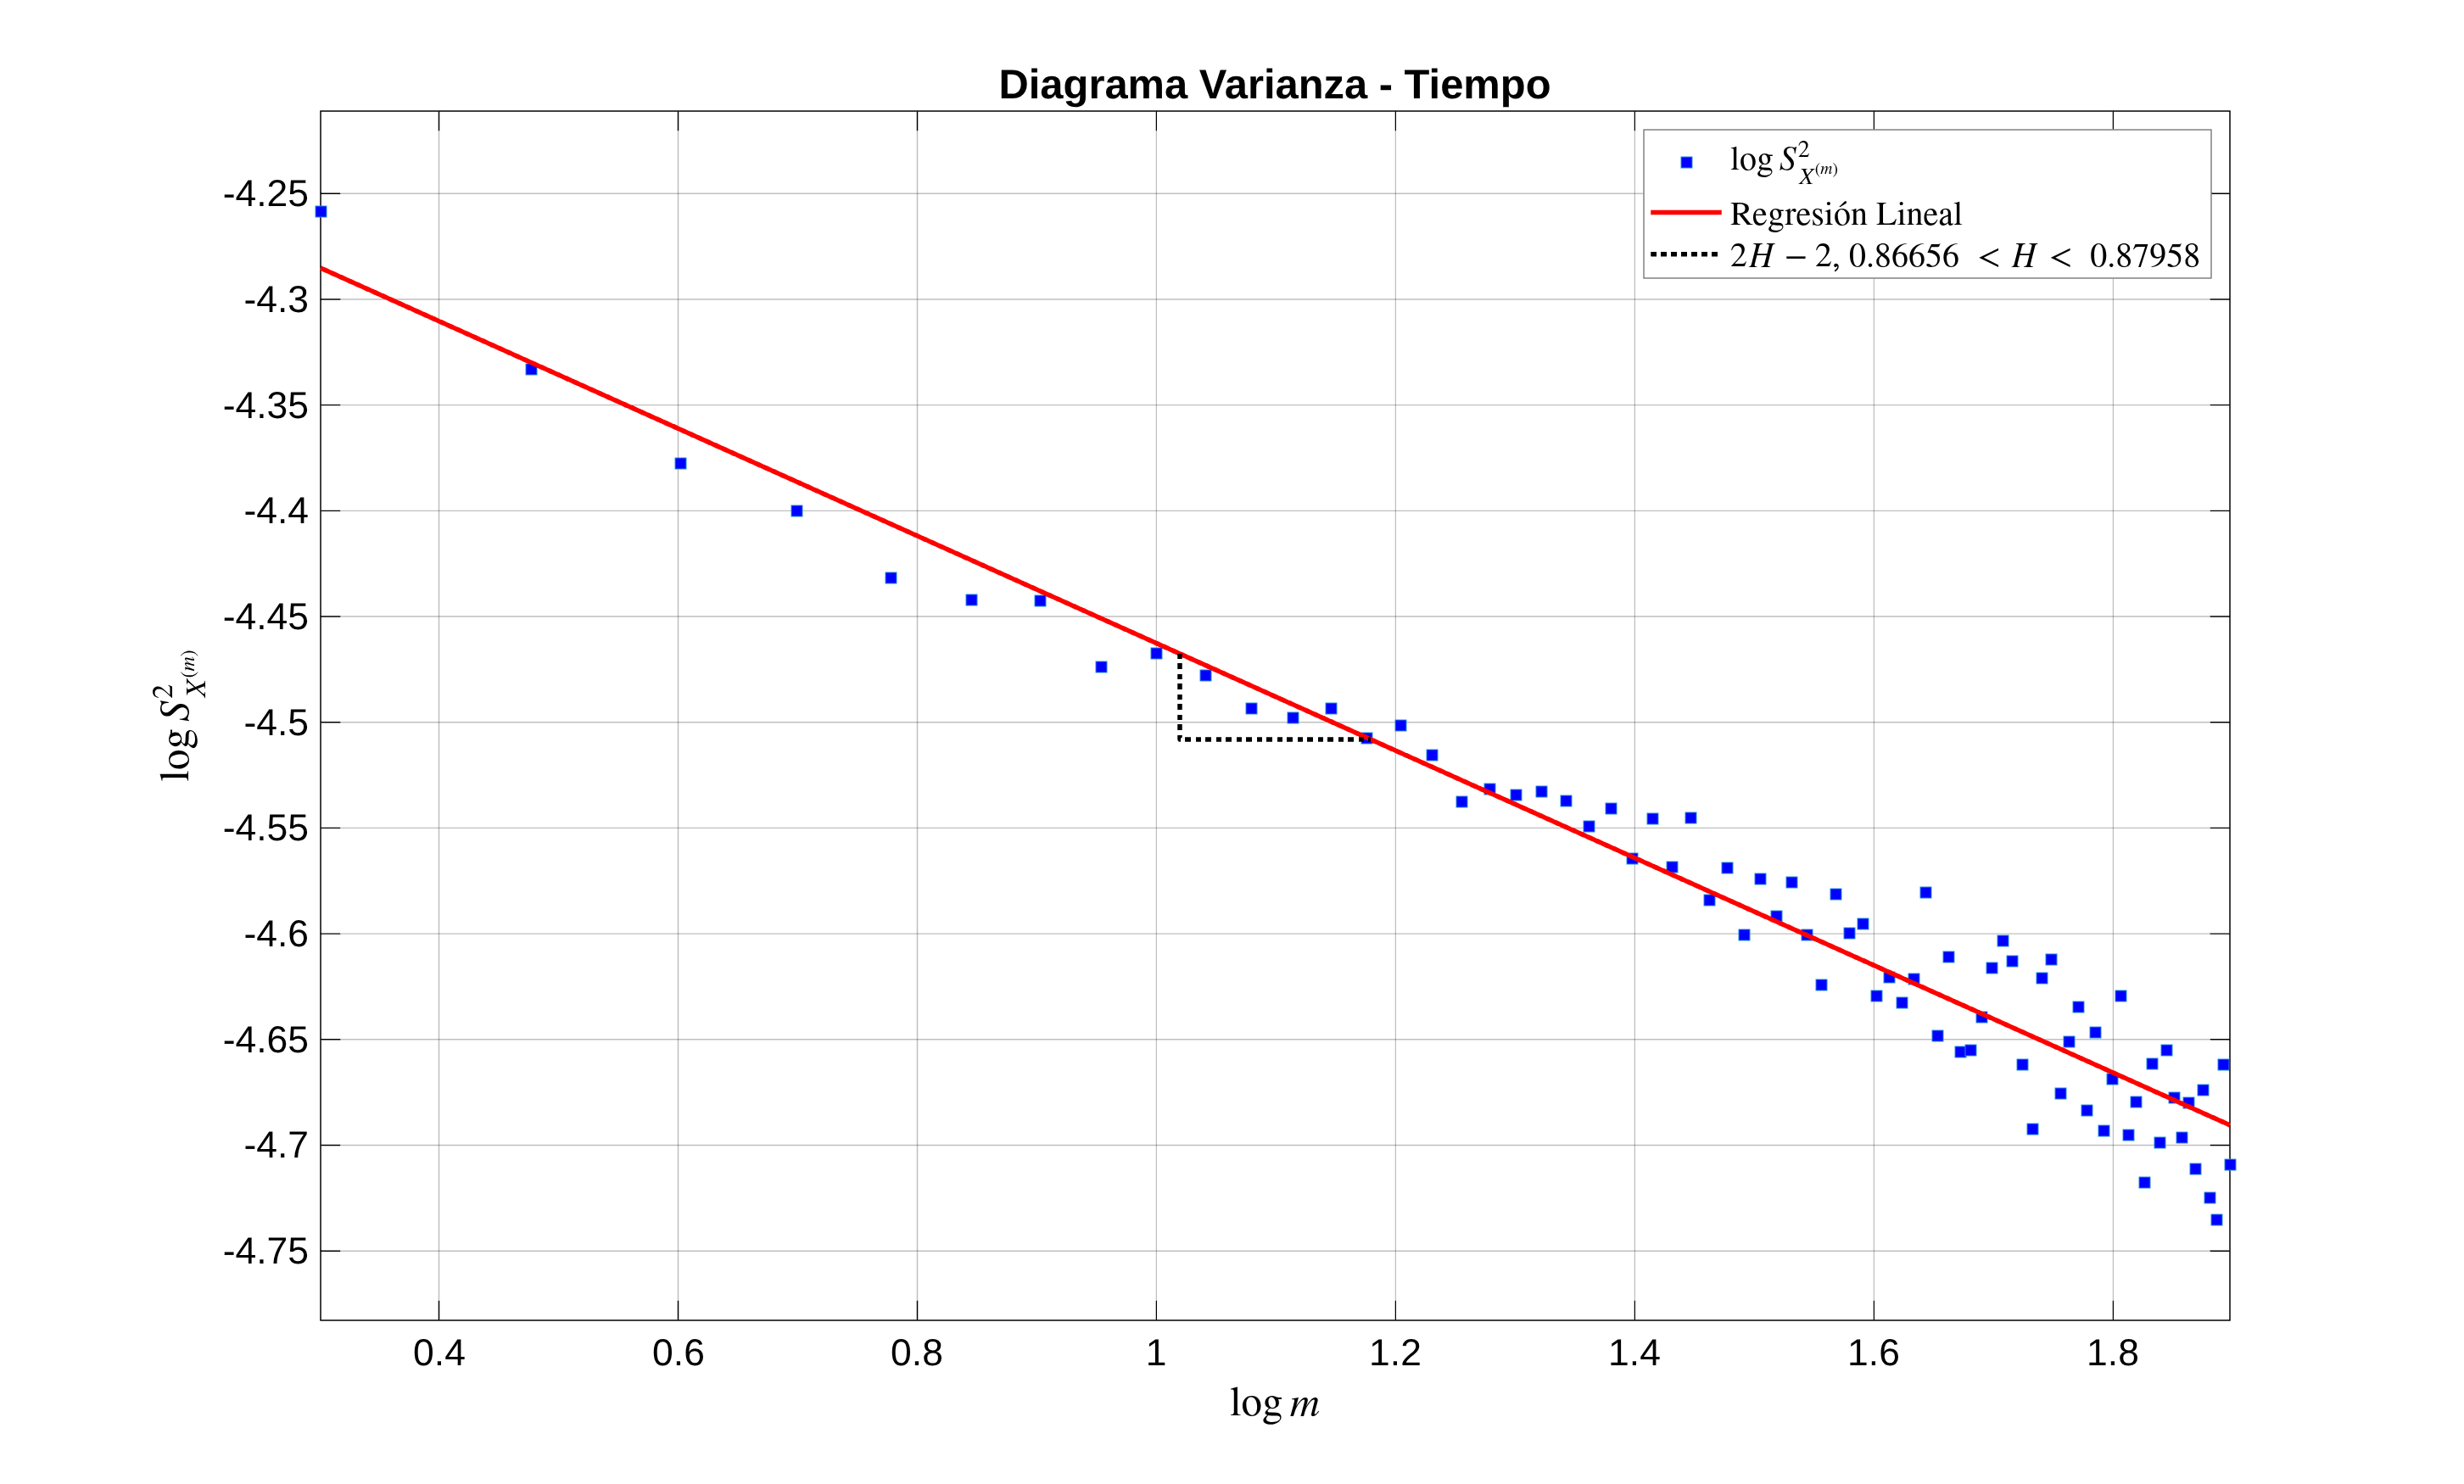
\includegraphics[width=0.85\textwidth]{actividades/actividad6/imgs/diagrama_vt.png}
    \caption{Diagrama de Varianza--Tiempo (VT). La pendiente del ajuste lineal determina $H = 0{,}5435$, significativamente por encima de $H_0 = 0{,}5$.}
    \label{fig:a6-vt}
\end{figure}

\subsubsection*{Método 2: Log--Escala --- ``El zoom que revela patrones ocultos''}

El método de Log--Escala (LD) detecta LRD mirando la energía de las fluctuaciones a diferentes escalas. Es como usar un microscopio con distintos aumentos para ver si una textura se parece a sí misma sin importar el zoom.

La idea es descomponer la señal en escalas (como las capas de una cebolla) y medir cuánta ``energía'' hay en cada una. En Poisson, la energía decae de forma predecible al aumentar la escala. En LRD, decae más lento porque las fluctuaciones grandes persisten.

\begin{figure}[H]
    \centering
    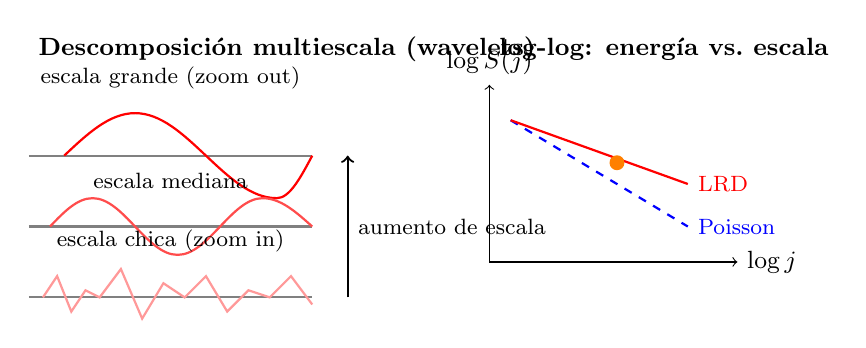
\begin{tikzpicture}[scale=0.9, every node/.style={font=\small}]
        % Zoom in / zoom out
        \node[anchor=west] at (0,3.5) {\textbf{Descomposición multiescala (wavelets)}};
        % Escala grande
        \draw[thick,gray] (0,2) -- (4,2);
        \draw[thick,red] (0.5,2) sin (1.5,2.6) cos (2.5,2) sin (3.5,1.4) cos (4,2);
        \node[above] at (2,2.8) {\footnotesize escala grande (zoom out)};
        % Escala mediana
        \draw[thick,gray] (0,1) -- (4,1);
        \draw[thick,red!70] (0.3,1) sin (0.9,1.4) cos (1.5,1) sin (2.1,0.6) cos (2.7,1) sin (3.3,1.4) cos (4,1);
        \node[above] at (2,1.4) {\footnotesize escala mediana};
        % Escala chica
        \draw[thick,gray] (0,0) -- (4,0);
        \draw[thick,red!40] (0.2,0) -- (0.4,0.3) -- (0.6,-0.2) -- (0.8,0.1) -- (1.0,0) -- (1.3,0.4) -- (1.6,-0.3) -- (1.9,0.2) -- (2.2,0) -- (2.5,0.3) -- (2.8,-0.2) -- (3.1,0.1) -- (3.4,0) -- (3.7,0.3) -- (4.0,-0.1);
        \node[above] at (2,0.5) {\footnotesize escala chica (zoom in)};
        % Flechas
        \draw[->,thick] (4.5,0) -- (4.5,2) node[midway,right,font=\footnotesize] {aumento de escala};

        % Mini gráfico log-log
        \begin{scope}[shift={(6.5,0.5)}]
            \node[anchor=west] at (0,3) {\textbf{log-log: energía vs.~escala}};
            \draw[->] (0,0) -- (3.5,0) node[right] {\small $\log j$};
            \draw[->] (0,0) -- (0,2.5) node[above] {\small $\log S(j)$};
            \draw[thick,blue,dashed] (0.3,2.0) -- (2.8,0.5) node[right,font=\footnotesize] {Poisson};
            \draw[thick,red] (0.3,2.0) -- (2.8,1.1) node[right,font=\footnotesize] {LRD};
            \fill[orange] (1.8,1.4) circle (3pt);
        \end{scope}
    \end{tikzpicture}
    \caption{LD descompone la señal en escalas con wavelets (izquierda). En log-log, la pendiente de LRD es menos empinada porque la energía persiste (derecha).}
    \label{fig:a6-concepto-ld}
\end{figure}

\texttt{LD.m} usa wavelets de Haar, grafica $\log(\text{energía})$ vs.~$\log(\text{escala})$ y la pendiente estima $H$.

Resultado: $\hat{H} = 0{,}5064$, $\alpha = 0{,}0127$. Consistente con VT, aunque más conservador ---algo que ya vimos en la Actividad~1, donde LD mostró mayor varianza en muestras grandes.

\begin{figure}[H]
    \centering
    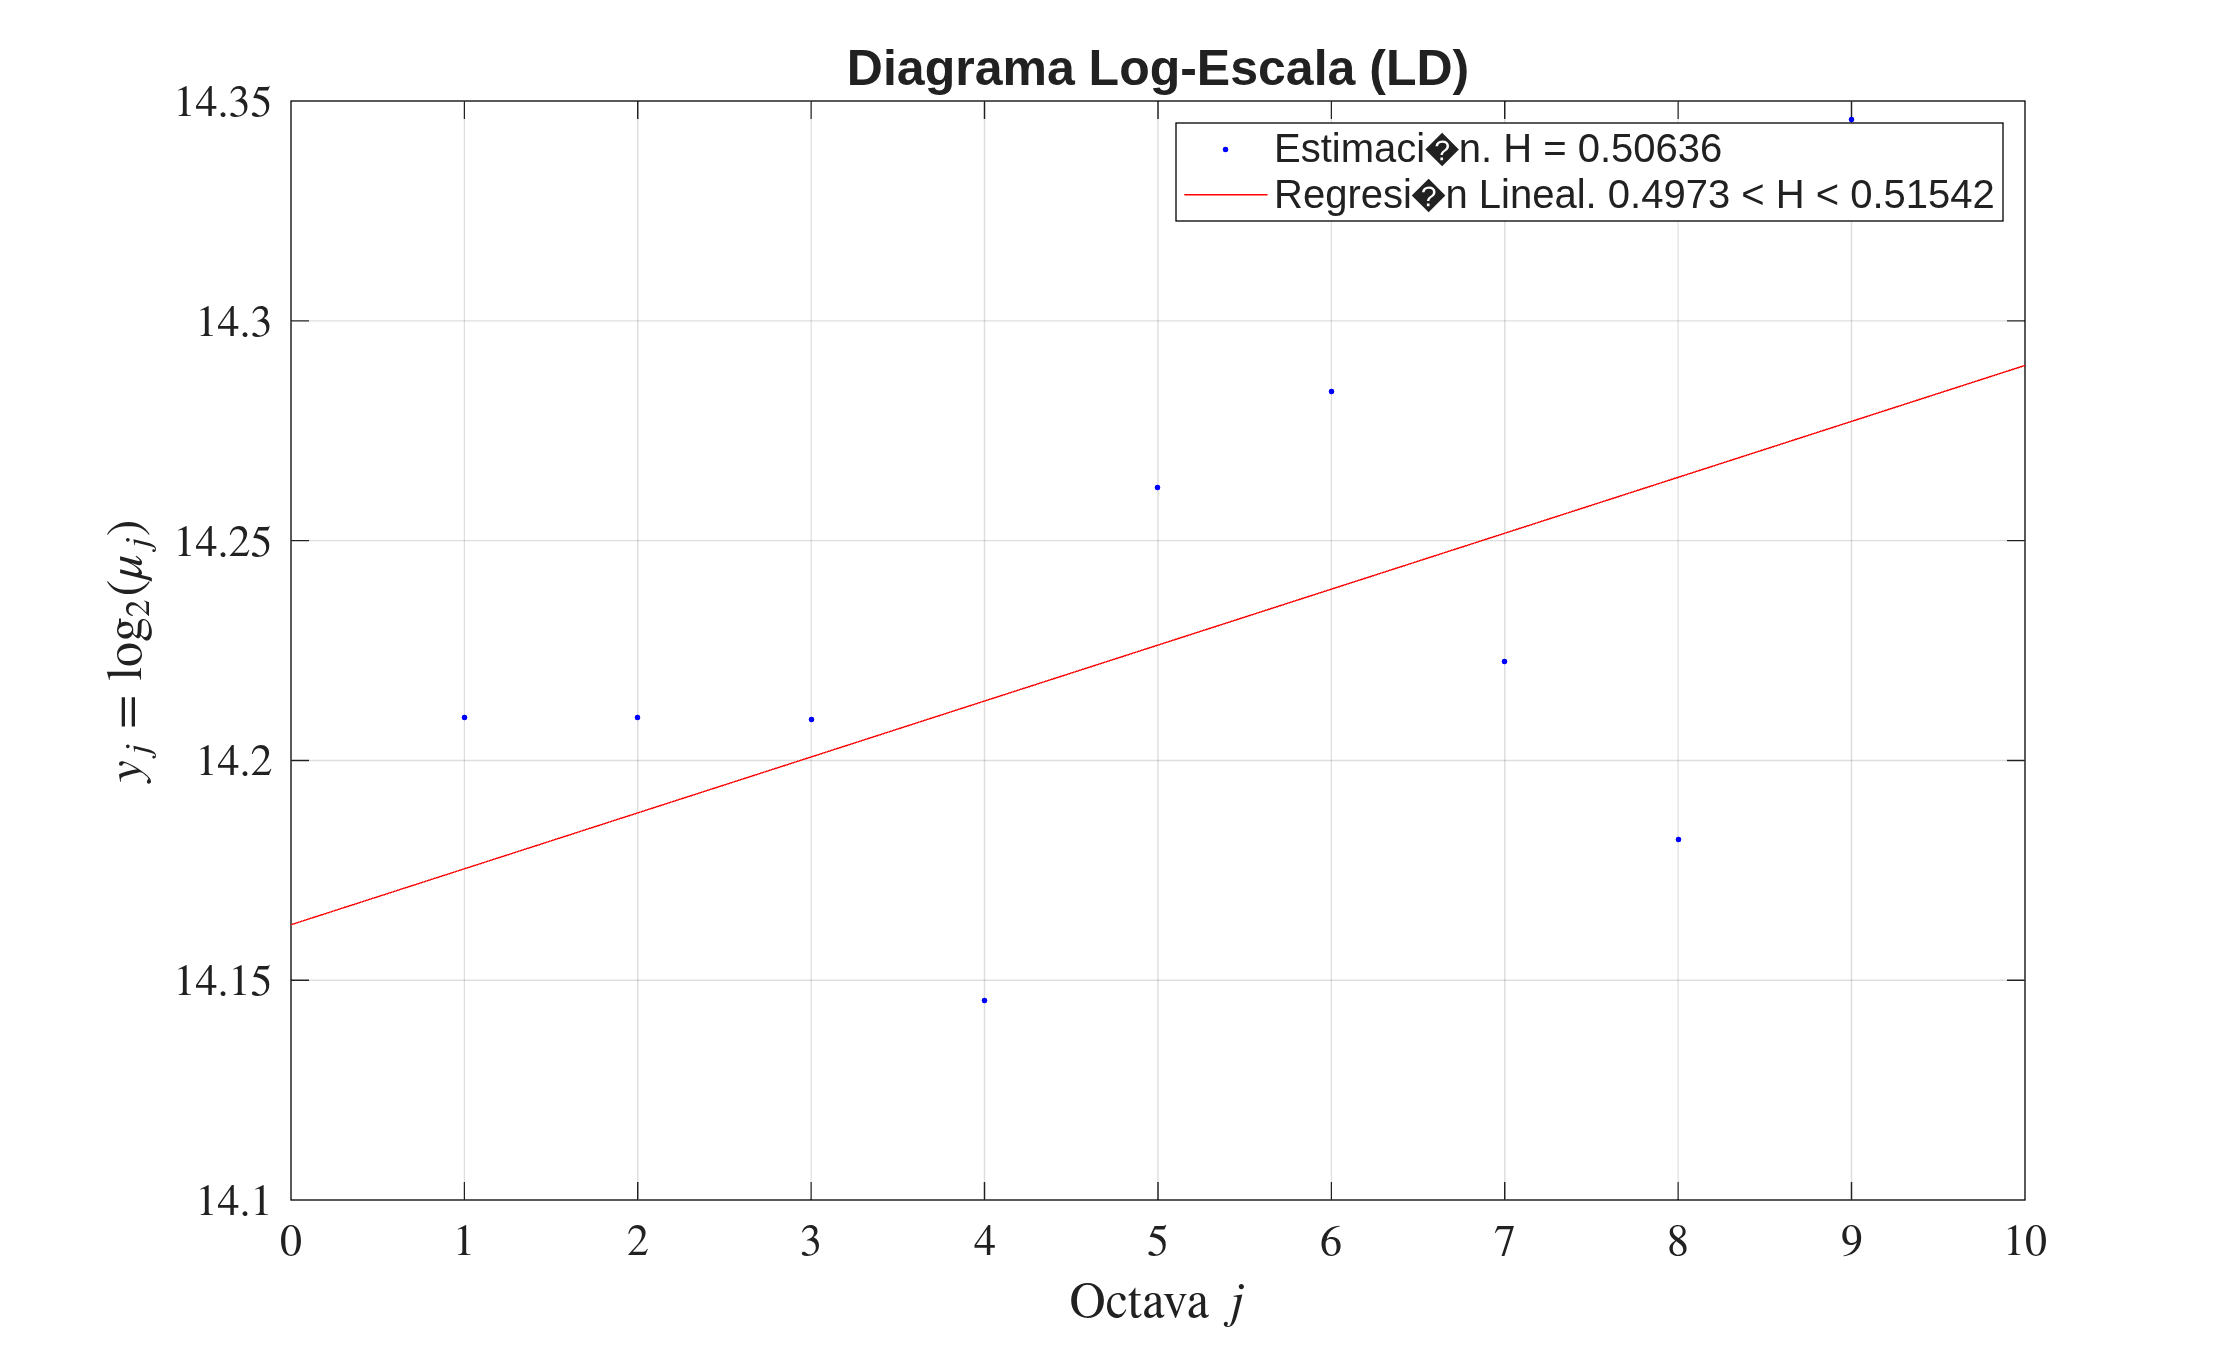
\includegraphics[width=0.85\textwidth]{actividades/actividad6/imgs/diagrama_ld.png}
    \caption{Diagrama log--escala (LD) con wavelets de Haar. Confirma LRD con $H = 0{,}5064$.}
    \label{fig:a6-ld}
\end{figure}

\subsubsection*{Clasificación: ¿Mono o multifractal?}

No todo proceso con LRD es igual. Hay dos tipos:

\begin{itemize}[leftmargin=2em]
    \item \textbf{Monofractal}: $H$ es el mismo en toda la serie. Es como una autopista donde el tráfico se comporta igual de caótico en todos los tramos.
    \item \textbf{Multifractal}: $H$ varía según la zona de la serie. Es como una ciudad donde algunas calles tienen tráfico caótico ($H$ alto) y otras están tranquilas ($H$ bajo).
\end{itemize}

\begin{figure}[H]
    \centering
    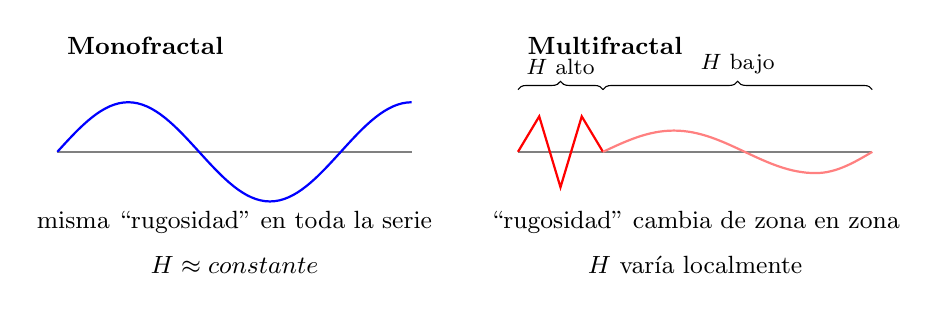
\begin{tikzpicture}[scale=0.9, every node/.style={font=\small}]
        % Panel izquierdo: monofractal
        \node[anchor=west] at (0,3) {\textbf{Monofractal}};
        \draw[thick,gray] (0,1.5) -- (5,1.5);
        \draw[thick,blue] (0,1.5) sin (1,2.2) cos (2,1.5) sin (3,0.8) cos (4,1.5) sin (5,2.2);
        \node at (2.5,0.5) {misma ``rugosidad'' en toda la serie};
        \node at (2.5,-0.1) {$H \approx \text{constante}$};

        % Panel derecho: multifractal
        \begin{scope}[shift={(6.5,0)}]
            \node[anchor=west] at (0,3) {\textbf{Multifractal}};
            \draw[thick,gray] (0,1.5) -- (5,1.5);
            % Zona rugosa
            \draw[thick,red] (0,1.5) -- (0.3,2.0) -- (0.6,1.0) -- (0.9,2.0) -- (1.2,1.5);
            % Zona suave
            \draw[thick,red!50] (1.2,1.5) sin (2.2,1.8) cos (3.2,1.5) sin (4.2,1.2) cos (5,1.5);
            \node at (2.5,0.5) {``rugosidad'' cambia de zona en zona};
            \node at (2.5,-0.1) {$H$ varía localmente};
            % labels
            \draw[decorate,decoration={brace,amplitude=3pt,raise=2pt}] (0,2.3) -- (1.2,2.3) node[midway,above=4pt,font=\footnotesize] {$H$ alto};
            \draw[decorate,decoration={brace,amplitude=3pt,raise=2pt}] (1.2,2.3) -- (5,2.3) node[midway,above=4pt,font=\footnotesize] {$H$ bajo};
        \end{scope}
    \end{tikzpicture}
    \caption{Monofractal: un solo $H$ gobierna toda la serie. Multifractal: diferentes regímenes de escalamiento coexisten.}
    \label{fig:a6-concepto-multi}
\end{figure}

\texttt{clasificar\_fractal.m} compara VT y LD y analiza la curvatura de $\tau(q)$:
\begin{itemize}[leftmargin=2em]
    \item Si $H_{\text{VT}} \approx H_{\text{LD}}$ y $\tau(q)$ es lineal $\rightarrow$ monofractal.
    \item Si divergen y $\tau(q)$ es curvo $\rightarrow$ multifractal.
\end{itemize}

Resultado: $R^2_{\tau} = 0{,}4808$ (muy por debajo de $0{,}90$). El tráfico NASA es \textbf{multifractal}: hay momentos de alta persistencia (ráfagas intensas) y momentos de baja persistencia (tráfico estable).

\begin{figure}[H]
    \centering
    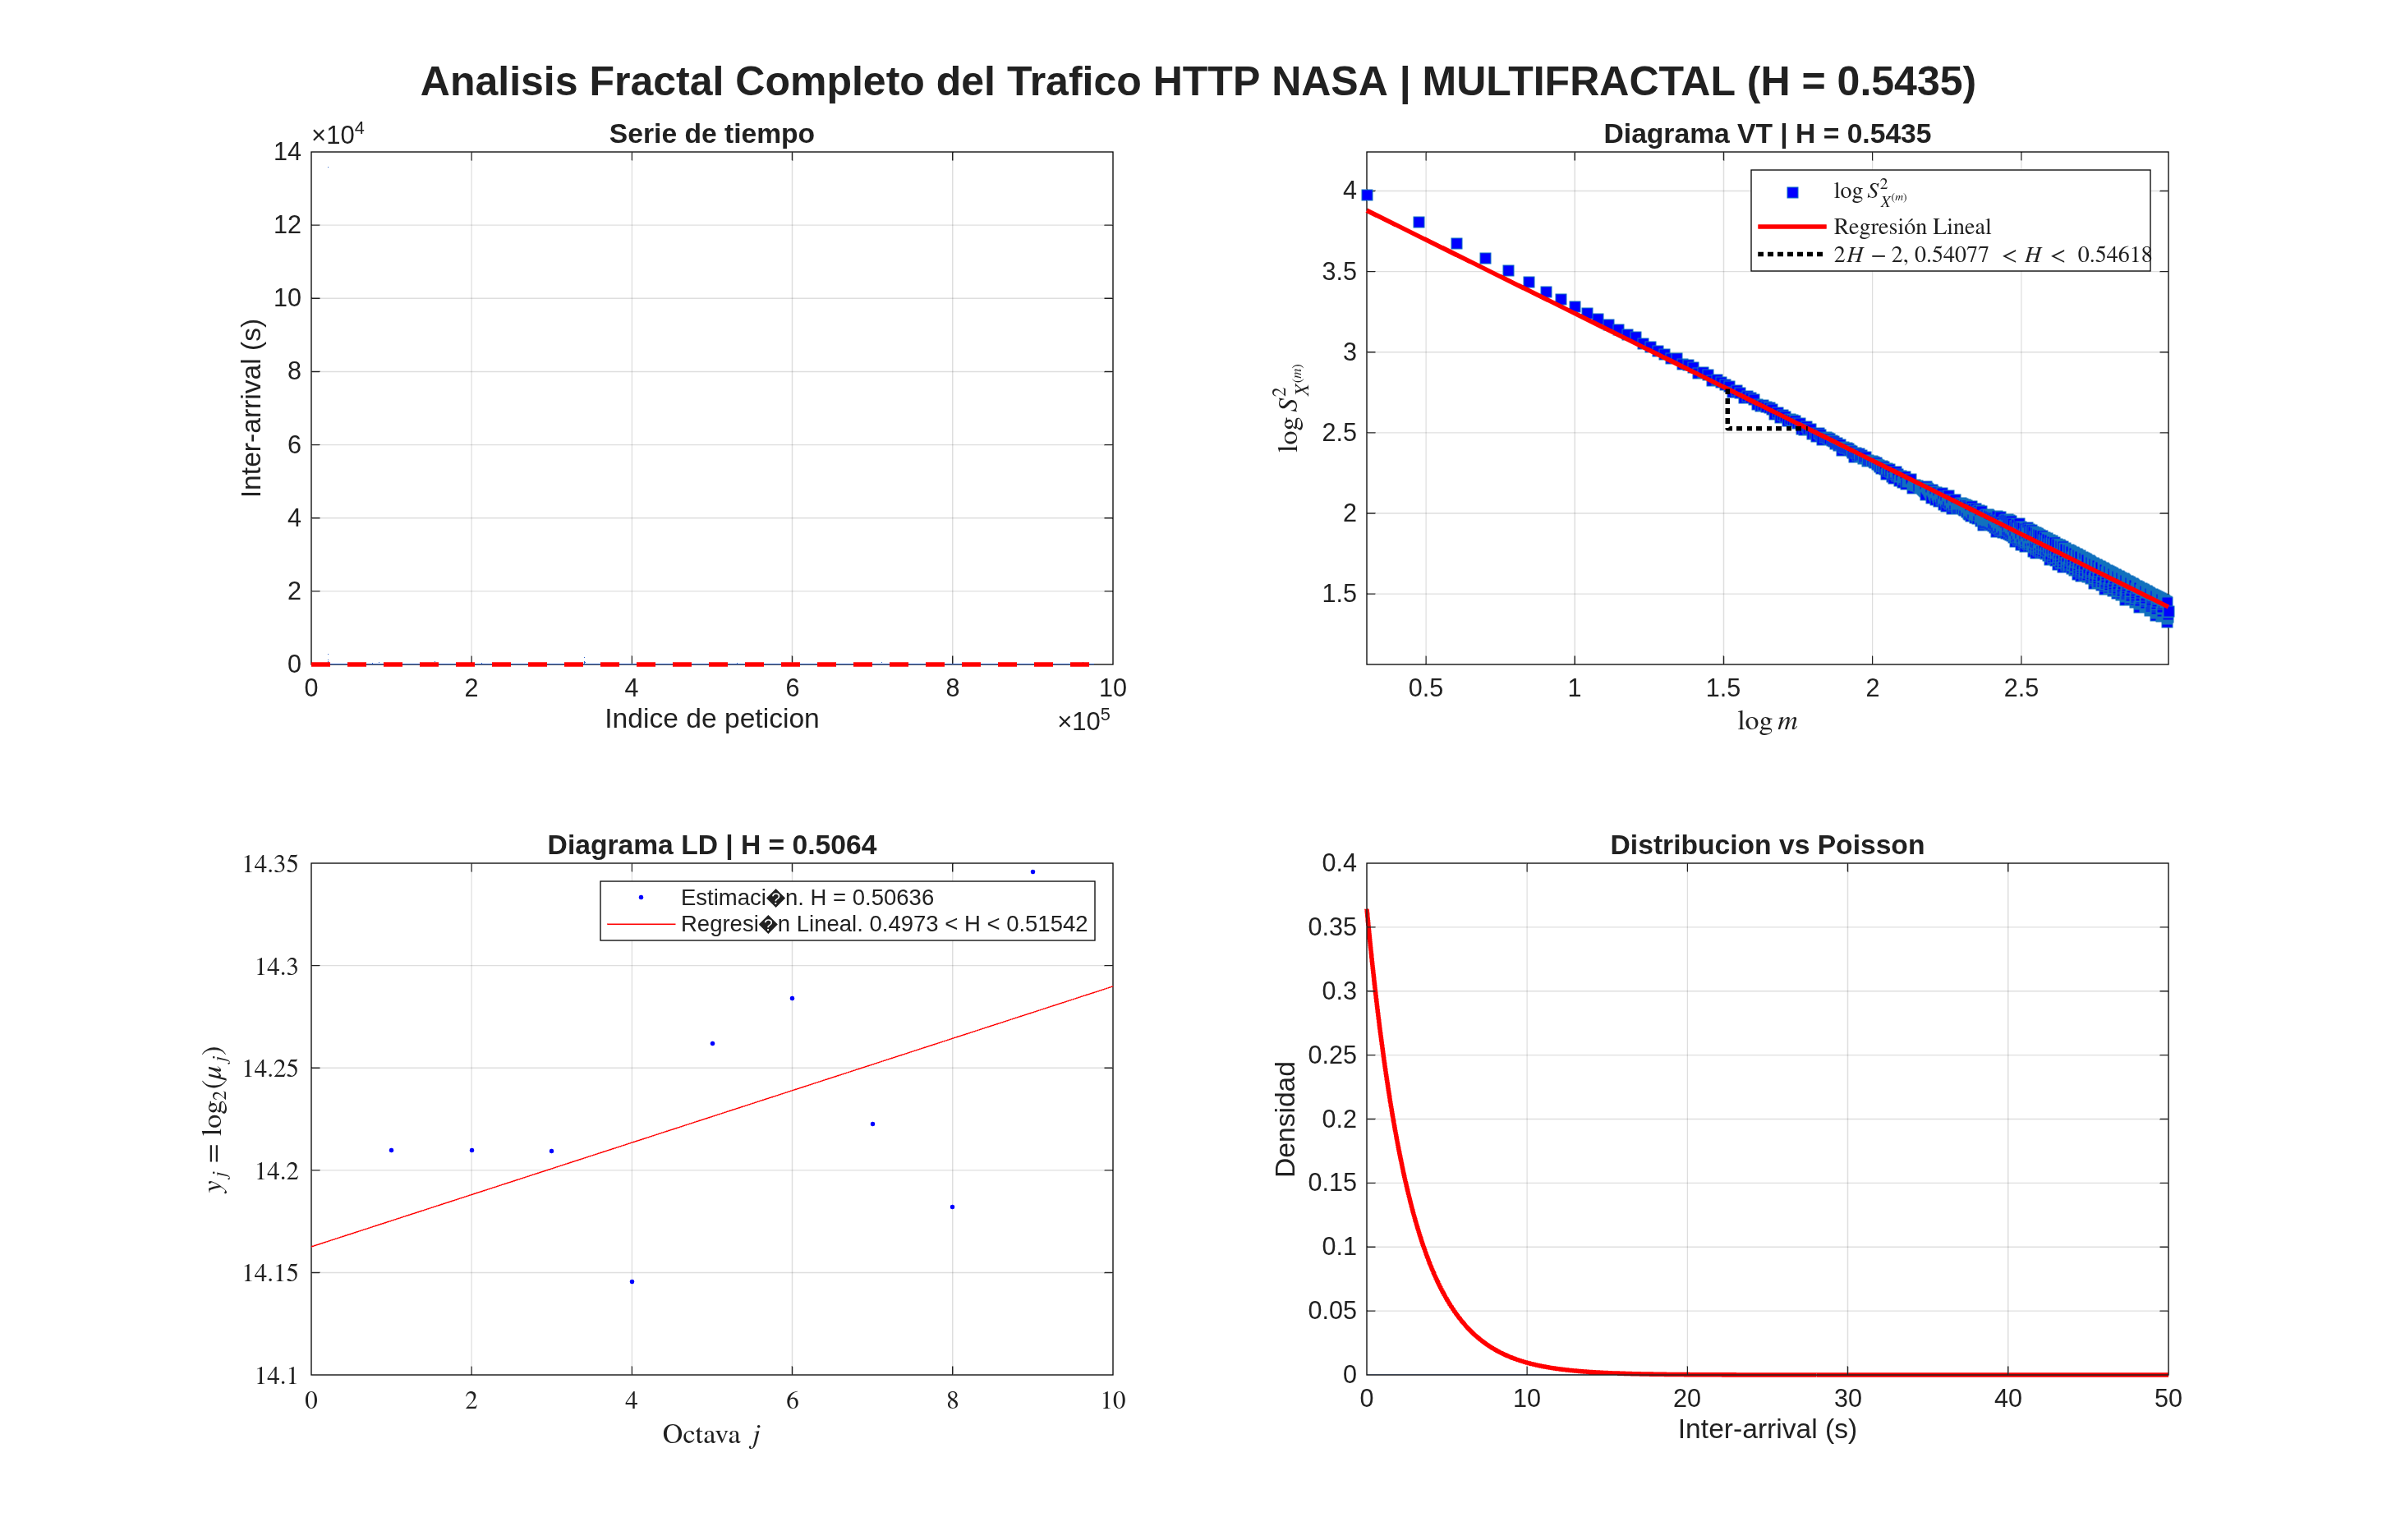
\includegraphics[width=\textwidth]{actividades/actividad6/imgs/panel_completo.png}
    \caption{Panel integrado: serie de tiempo, diagrama VT ($H = 0{,}5435$), diagrama LD ($H = 0{,}5064$) y distribución vs.~Poisson.}
    \label{fig:a6-panel}
\end{figure}

\subsubsection*{Implicaciones para la orquestación Cloud}

¿Por qué importa esto? Si diseñamos servidores, CDNs o políticas de auto-escalado asumiendo Poisson, vamos a subestimar las colas, vamos a subestimar los picos de congestión, y vamos a diseñar una infraestructura que se cae en las horas pico. Es como diseñar una autopista asumiendo que los autos llegan uno por uno perfectamente espaciados, cuando en realidad vienen en caravanas.

El parámetro de Hurst nos da una herramienta cuantitativa para medir esa memoria y tomar decisiones de infraestructura más inteligentes: reservar capacidad antes de que llegue la ráfaga, en lugar de reaccionar cuando ya es tarde.
